%! Anhang

\clearpage
\appendix
\clearpage

%! Chapter Befehl wird umgeschrieben, um Überschriften zu verbergen
%! Kann, falls Überschriften gewollt sind, entfernt oder erst später eingefügt werden.
% Beginn
\makeatletter
\renewcommand{\chapter}[1]{%
\par\refstepcounter{chapter}%
\sectionmark{#1}%
\NR@gettitle{#1}%<---------
\addcontentsline{atoc}{chapter}{\bfseries\protect\numberline{\thechapter}{\mdseries#1}}%
\lohead{\textnormal{#1}}%
}
\makeatother
% Ende

%! Anpassung der Darstellung von Abbildungen im Anhang
%! Eine Variante auskommentieren
%? Möglichkeit 1: ohne Nummerierung
%\renewcommand{\bild}[4][1.0]{\begin{figure}[H]
    %\centering
    %\includegraphics[width=#1\columnwidth]{bilder/#2}
    %\caption*{\bfseries Abbildung \mdseries #3}
    %\label{#4}
    %\end{figure}}

%? Möglichkeit 2: mit Nummerierung aber nicht im Abbildungsverzeichnis
\renewcommand{\bild}[4][1.0]{\begin{figure}[H]
    \centering
    \includegraphics[width=#1\columnwidth]{bilder/#2}
    \caption[]{#3}
    \label{#4}
    \end{figure}}

%! CD/USB-Inhalt, für USB-Stick entsprechend anpassen, Icon ein-/ CD ausblenden
\chapter{Inhalt der CD}
\label{cd-inhalt}
\renewcommand\DTstyle{\sffamily}
\renewcommand{\DTstyle}{\textrm\expandafter\raisebox{-0.7ex}}
\dirtree{%
.1 
%! CD
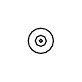
\begin{tikzpicture}
    \draw circle (0.16);
    \draw circle (0.07);
    \draw circle (0.02);
\end{tikzpicture}
%! USB
%\hspace{.2em}\dtusb
\raisebox{.05em}{ CD mit folgenden Inhalten:}.
.2 \dtfolder Anhänge.
.2 \dtfolder LaTeX-Quellen.
.2 \dtfolder Online-Quellen.
.2 \dtfile dieses Dokument.
.2 \dtfile \href{https://www.youtube.com/watch?v=dQw4w9WgXcQ}{YouTube-Video} als Bonus.
}
\vspace*{\fill}
\begin{center}
    \begin{tikzpicture}
        \draw (0,0) rectangle (12.2,12.2);
        \draw (6.1,6.1) circle (5.5);
        \draw (6.1,6.1) circle (.75);
        \draw (6.1,6.1) circle (2.4);
    \end{tikzpicture}
\end{center}
\vspace*{\fill}
\clearpage

% Warnungen für vorgefertigte Dokumente deaktivieren
\hbadness=10000
% Eidesstattliche Erklärung, Erklärung Plagiatsprüfung
\input{vorlage/Erklärung}

% Warnungen zurücksetzen
\hbadness=1000